% !TEX root = ../../thesis.tex

\cleartoleftpage
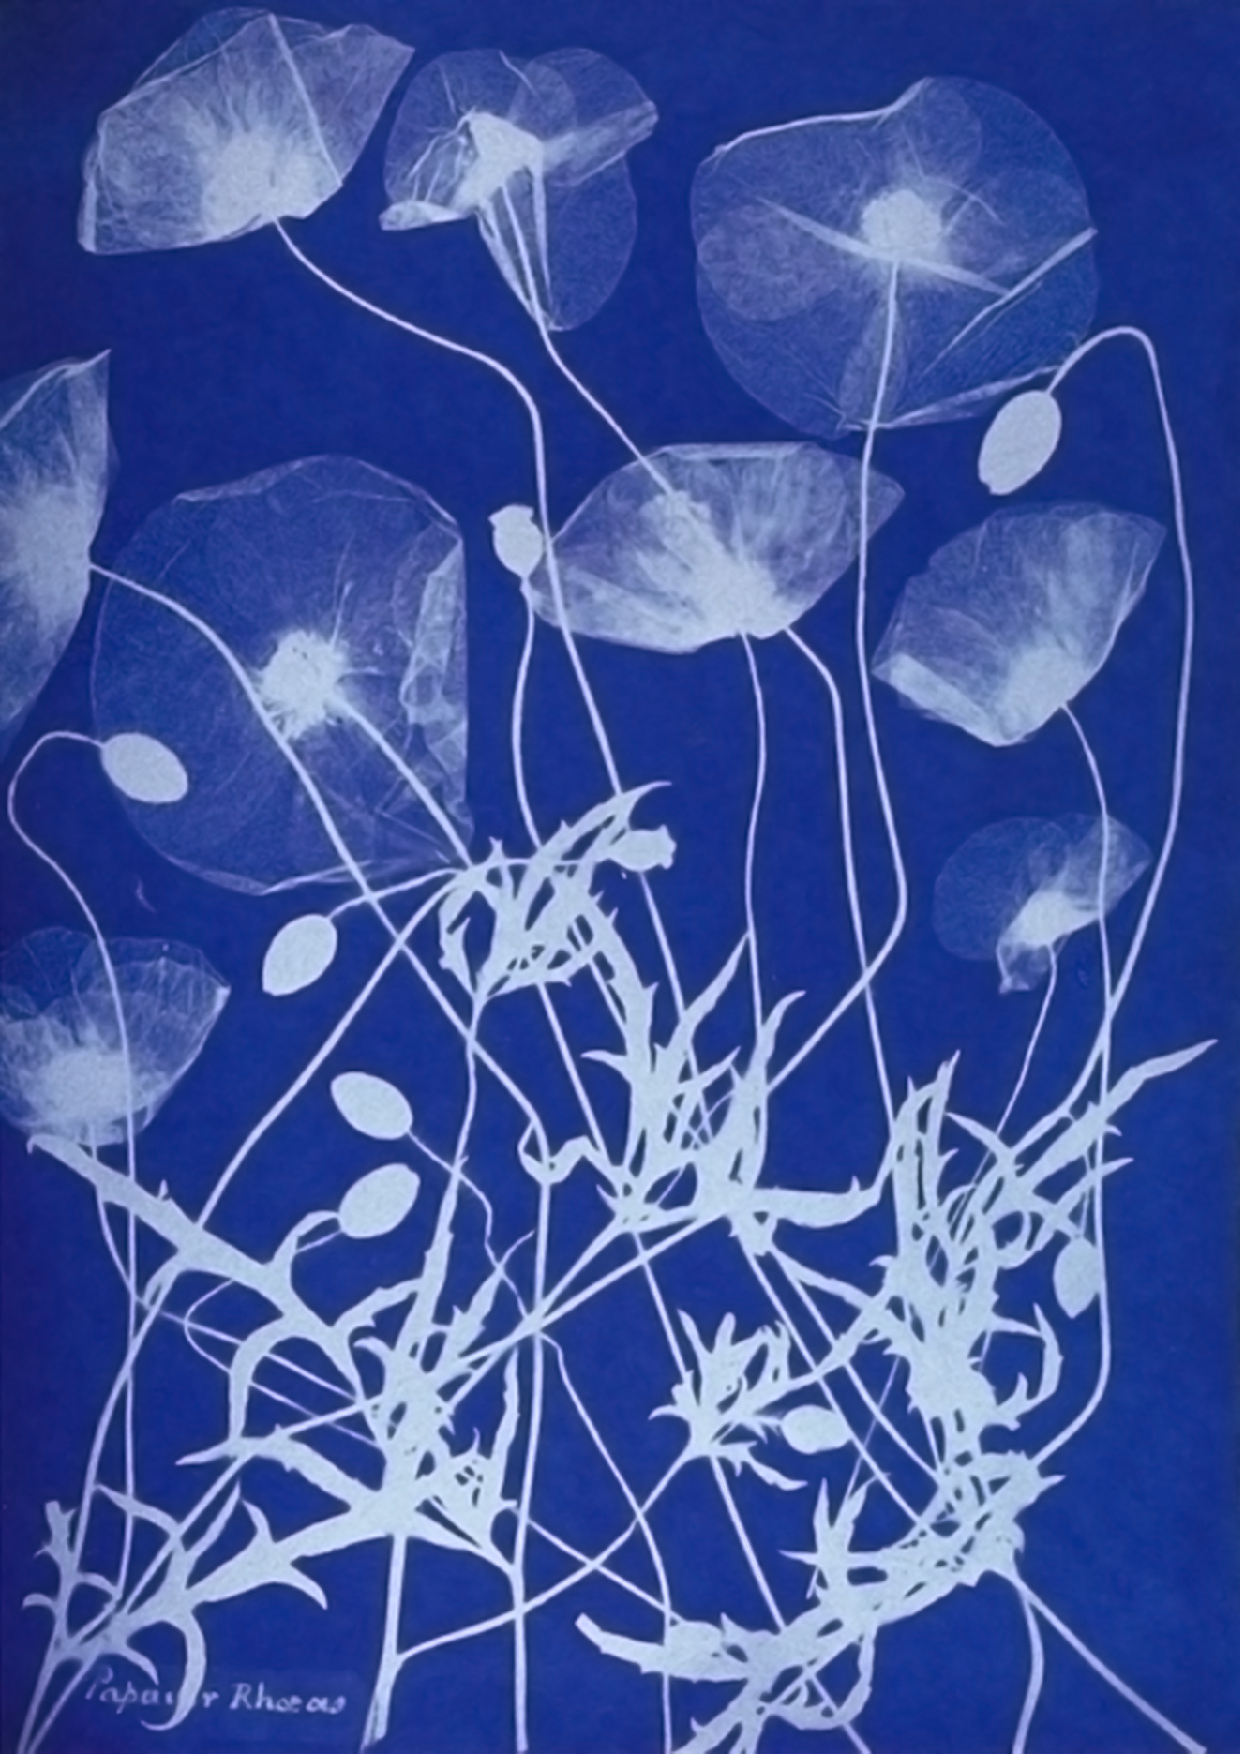
\includepdf{../media/chapter_illustration/papaver_rhoeas}



\chapter{The Poppy development} % (fold)


\section{Introduction} % (fold)

Research in humanoid robotics has been thriving in the recent years~\cite{hirai1998development} \cite{kaneko2008humanoid}, both due to theirs predicted relevance for personal and assistive robotics~\cite{tapus2007socially} \cite{oztop2005human}, and because of the scientific challenges raised by robotics with regards to cognition~\cite{asada2001cognitive}, natural communication~\cite{stiefelhagen2004natural} \cite{breazeal2002robots}, biped locomotion~\cite{yamaguchi1999development} \cite{chestnutt2005footstep} \cite{collins2005bipedal} and full-body physical interaction with the environment~\cite{ude2004programming}.

But like the LHC is an experimental platform allowing to explore quantum mechanics and the origin of our universe,  humanoid can act as simplified and controllable human simulator. Thus humanoid robots can be amazing tools to study human-being and eventually contribute in a better understanding of Human's behaviors and abilities~\cite{atkeson2000using} \cite{cheng2007cb} \cite{brooks1986achieving}.

A famous example of such humanoid uses was the Cog project~\cite{brooks1999cog} at the Humanoid Robotics Group of the Massachusetts Institute of Technology. This research project has two goals: an engineering goal of building a prototype general purpose flexible and dextrous autonomous robot and a scientific goal of understanding human cognition~\cite{brooks1994building}. In particular, this project concentrated on embodiment and interaction intelligence with four aspects of a novel methodology: developmental structure, physical embodiment, integration of multiple sensory and motor systems, and social interaction. For this purpose they build several robotic platform such a humanoid~\cite{brooks1999cog} (see \figurename~\ref{fig:brooks_and_cog}), and a very expressive multi-articulated head named Kismet~\cite{breazeal2003emotion} (see \figurename~\ref{fig:breazeal_kismet}).

% This project ended in 2003 and has bring great scientific contributions such as ... REF


\begin{figure}[t]
\centering
    \subfloat[][Rodney Brooks and the Cog humanoid]{\label{fig:brooks_and_cog}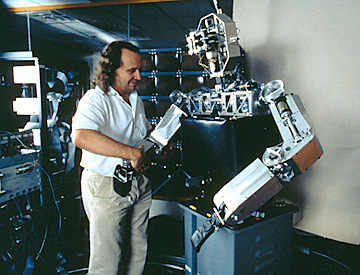
\includegraphics[height=5cm]{brooks_and_cog.jpg}}
    \hfil
    \subfloat[][Cynthia Breazeal with Kismet]{\label{fig:breazeal_kismet}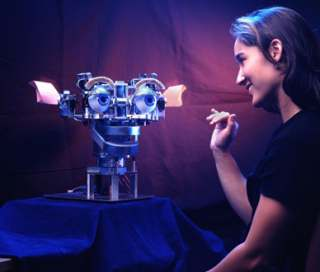
\includegraphics[height=5cm]{breazeal_kismet.jpg}}
    \caption{The Cog project was about the use of computer and robotic technology to better understand and emulate human intelligence.}
    \label{fig:cog_project}
\end{figure}



The context of this PhD thesis is grounded on the same scientific motivations as the work of R.Brooks, R.Pfeifer, T.McGeer and initiative such as the Cog project i.e. exploring the role of morphology, cognition and embodiment intelligence in several aspects using real experimental robotic platforms.

The scientific approach of the Cog robots is oriented toward the exploration of embodiment in several aspects, from the low level mechatronics to head design for social interactions, but they were built 15 years ago and using classic manufacturing technique (see \figurename~\ref{fig:cog_project}) that made them expansive, complicated to be modified and especially difficult to diffuse in other laboratories.
We are now in 2014, the makers revolution is in progress~\cite{anderson} and novel technologies allows to rethink the way we design robotic platforms, especially humanoid.

In the previous chapter we presented a methodology to design robotic platform allowing both a free exploration of morphological variations and the diffusion in the research community. This method uses 3D printing to produce mechanical part, Arduino architecture for the electronic system and python-based API for the control.

We think such design methodology can contribute in building better experimental robots while it allows to make the modification of a robot morphology both easy and low cost, and by the use of open source diffusion, it permits the transfer and the reuse of scientific work in other laboratories.
Within this context we built a whole new humanoid robot called PoppyTM (see Fig.~\ref{fig:poppy_with_me}).

\begin{figure}[tb]
    \begin{center}
        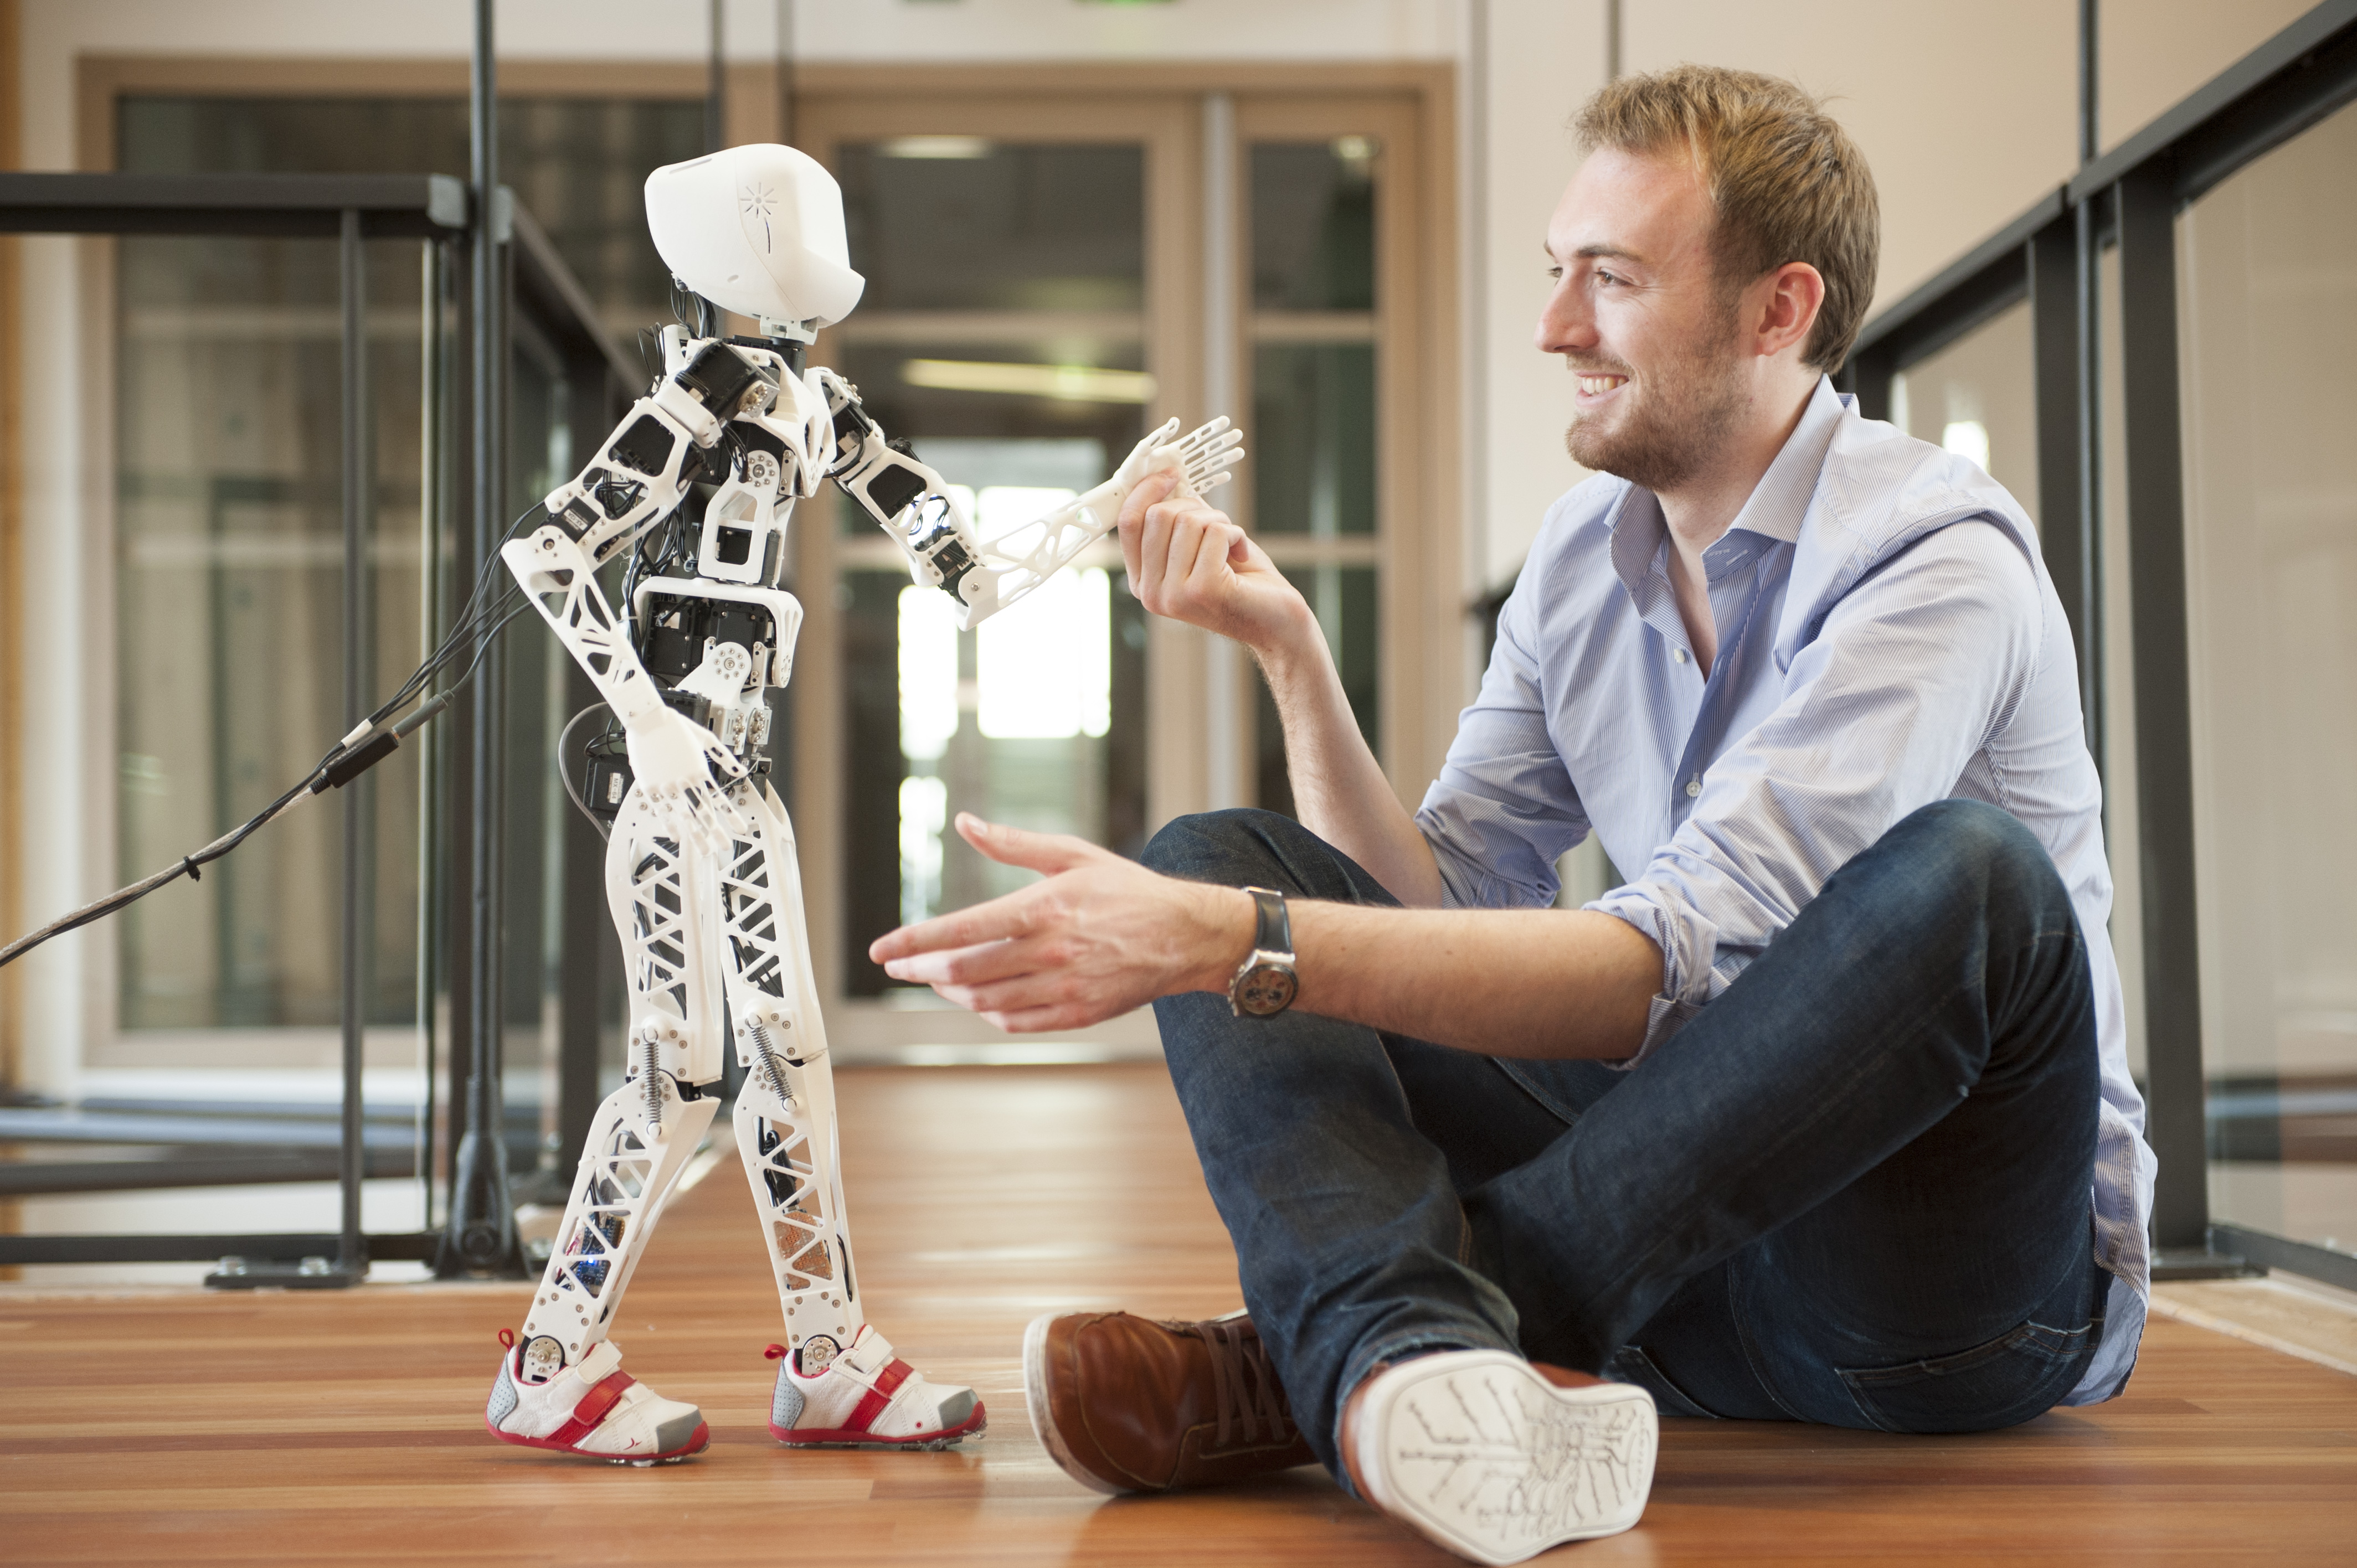
\includegraphics[width=0.7\linewidth]{lapeyre_and_poppy.jpg}
    \end{center}
    \caption{Poppy}
    \label{fig:poppy_with_me}
\end{figure}

This humanoid robot is designed to easily and quickly conduct scientific experiments on sensorimotor learning, exploring morphological properties, and human-robot interaction. As an experimental robotic platform, Poppy is designed to be \textbf{affordable}, \textbf{lightweight}, \textbf{robust and safe}, \textbf{easy to use}, \textbf{highly-hackable} and \textbf{fast and easy to duplicate or modify} with the goal to be easily reproducible and used by other lab thanks to an open source distribution (hardware and software).

In this chapter,  we will describe our motivation, the design guidelines we have followed and the conception of Poppy.


\section{Creating a novel humanoid robot} % (fold)

\subsection{Motivations} % (fold)

In 2012, when we started this work, none of the existing humanoid platforms were suitable for exploring the role of morphology. There were two kind of platform. On one hand the commercial robots, rather easy to use and accessible but with a static and frozen morphology. On the other hand, prototype robots produced in labs to adresse specific experimentations, studying interesting morphologies but complicated to use and impossible to reproduce outside the lab.

In our lab, we had both kind of robot. We used Nao (see \figurename~\ref{fig:nao_platform}) to study human robot interaction (REF PIERRE cadeau). It was really convenient to be use by researchers those are not comfortable with get their hands dirty and do not really care about hardware issue while their are addressing more high-level research challenges. Yet such platform is limited as it is not possible to modify it if the robot is not adapted to our experiment. For example back at this time the Nao camera was not efficient, we have difficultly achieved 5 frames/seconds.
We had the necessary skills to hack Nao and change the camera but its hardware is not designed to be changed. Improving the vision performance could only be possible by the addition of an external camera on the Nao head which would ruin the user experience.

\begin{figure}[]
\centering
    \subfloat[][Nao]{\label{fig:nao_platform}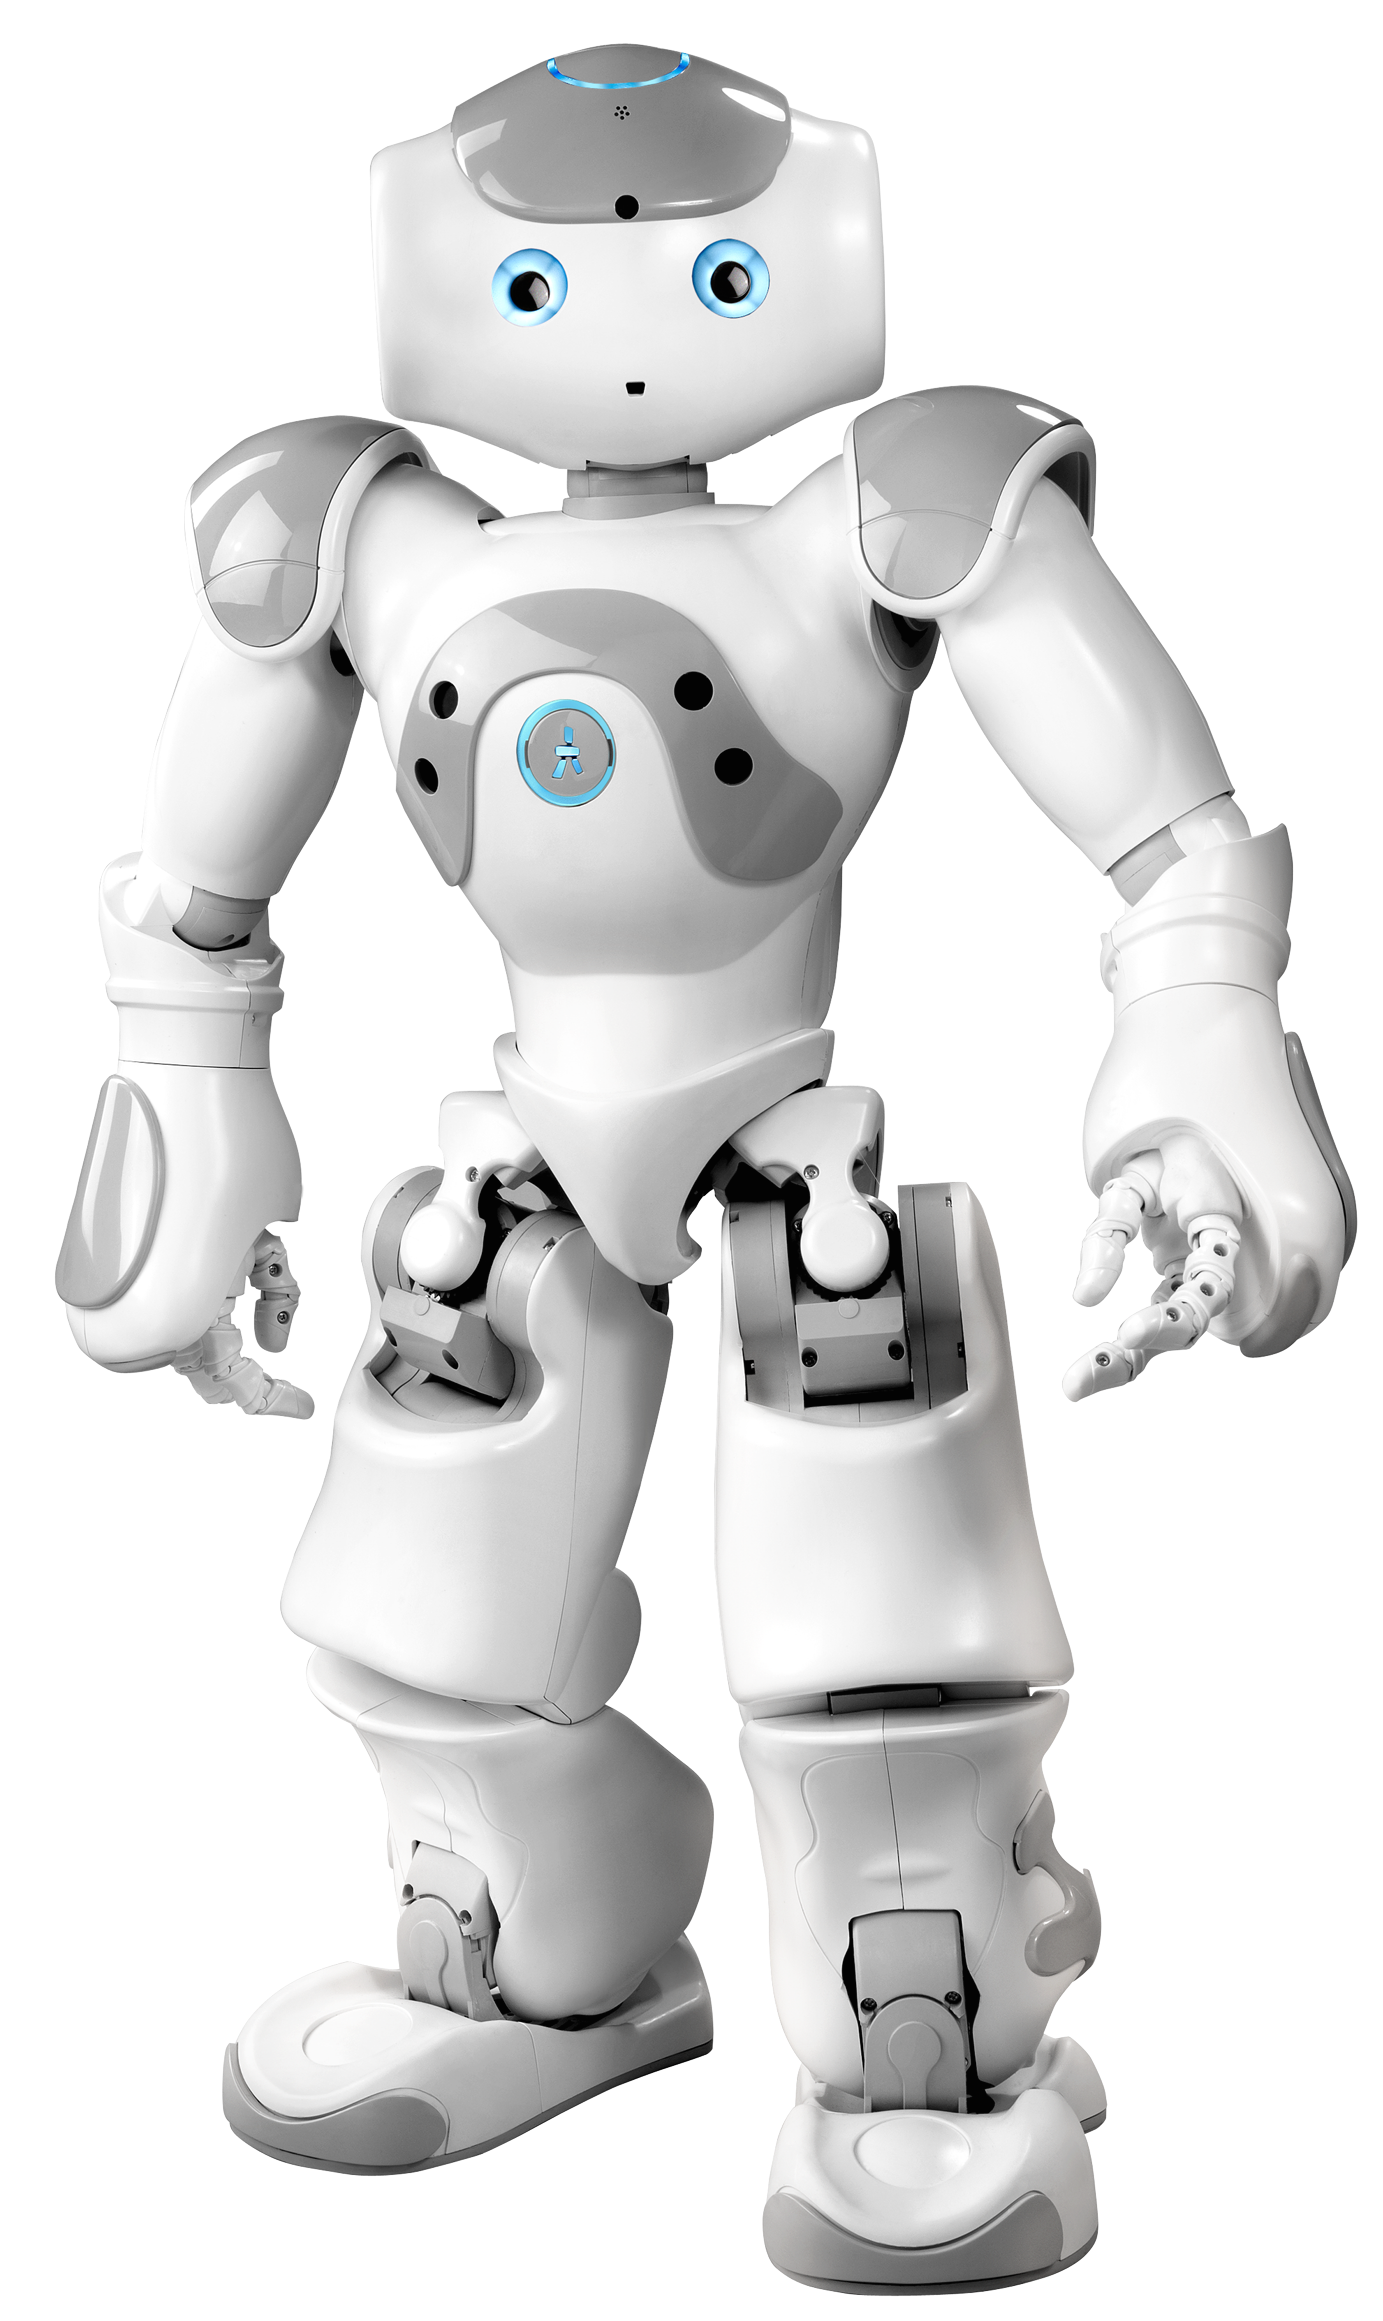
\includegraphics[height=5cm]{nao_face.png}}
    \hfil
    \subfloat[][Darwin-Op]{\label{fig:darwin_platform}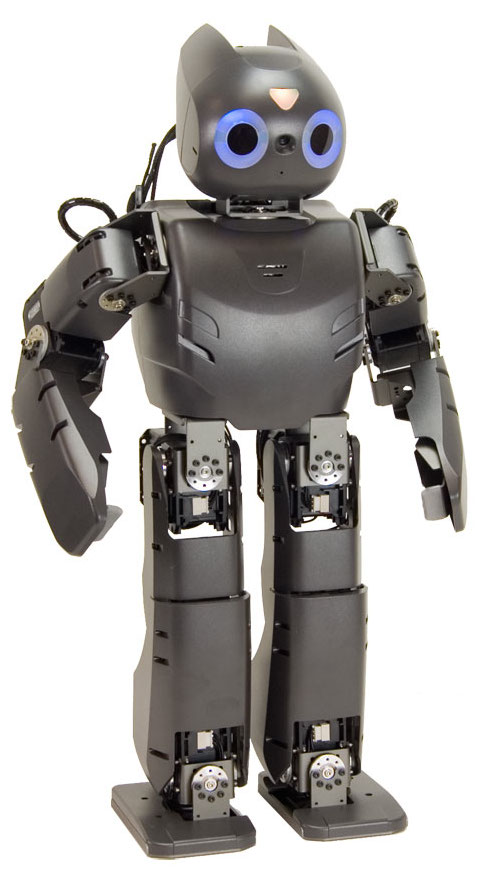
\includegraphics[height=5cm]{darwin_op_face.jpg}}
    \hfil
    \subfloat[][Acroban]{\label{fig:acroban_platform}\includegraphics[height=5cm]{acroban_wout_background.jpg}}
    \caption{None of the existing platform in 2012 was suitable to explore the role of morphology. Nao was impossible to modify. Darwin Op and Acroban used aluminium part really difficult and expensive to produce.}
    \label{fig:2012_Humanoids}
\end{figure}

We also used Acroban (see \figurename~\ref{fig:acroban_platform}) designed in our team by Olivier Ly~\cite{Ly2010}. It is a handcrafted humanoid platform created to explore morphological properties, especially compliance toward the achievement of dynamic locomotion and playful physical human robot interaction.
While it actually allows modification of its is morphology, its manufacture based on aluminum mechanical parts, Robotis Dynamixel motors, scotch, and rubber bands cobbled together therefore requires lot of effort to be changed. Especially the manufacture of aluminum parts require specific skills and tools.
Also its use was quite complicated and while several researchers could have been interested by Acroban to study human robot interaction and social acceptance, it was not possible to use it without getting our hands dirty.
Finally, the material and manufacture process make platform non-stationary, even if a lab manage to reproduce it, there is a high probability that the physical properties will not be the same. Therefore, the diffusion and the reproducibility of results are limited.


A last alternative would be the use of Darwin Op robot (see \figurename~\ref{fig:darwin_platform}) which is both open source and reproducible, yet as Acroban its hardware based on manufactured metal parts make its morphology difficult and expensive to be modified. Moreover to our knowledge, Darwin morphology has never be changed by the research community.

Thus one of the main goals was to achieve the design of a humanoid robot which can merge the advantages of both kind of robot, i.e. simple, accessible, reproducible and allowing to easily change and hack its morphology.

\subsection{A robot experiments-proof} % (fold)

Most researchers can attest of the difficulty and frustration raised by conducting robotic experimentation in the real world. We are daily challenged by bugs, technical issues, unpredicted events and side effects. While a bug in a software can be fixed, an error with a hardware platform can cause damages and postpone the results of an experiment by several weeks.

Therefore many robotic researchers avoid technical issues link with the real world experimentation by using simple model and physical simulation. But the real world is extremely more complex and rich than the virtual one.
Some high-level behavior experiments are conducted in simulator based on the hypothesis that the real world constraints are not relevant, yet it is really sure ?
Indeed, while the real world constitute a lot of constraints, it is also rich of complex physical effects (gravity, friction, inertia) which has to be took in and can be very useful if interacting with the agent.

As we saw in the related work (chapter~\ref{REF}), the emergence of complex behavior can appear thanks to the interaction between the real world and simple robotic system. We cannot program behavior while the behavior is the interaction resultant between the program and the real world. Thus we cannot design behavior without the ecological niche of the robot~\cite{Steels1991emergence}.

While using simulator can be helpful as a first step to design robot, it appears incomplete to show results on the role of morphology without real world experimentations.
Therefore, when ones want to study the role of morphology on the robot behavior, being able to explore it in the real world is of paramount importance.

Along our work on building cognitive and developmental learning algorithms, we had experienced these issues, especially while building and using Acroban~\cite{Ly2010} and during the Ergo robot experience (see section~\ref{REF}).

Therefore Poppy has been designed based on the experience background we have building and using robots acting in the real world.

\begin{description}
    \item[Robustness and Safety:] Heavy and long real-world experimentations imply a robot should be robust and safe. It should be able to sustain experiments and fall down without easily breaking. At the same time, one should ensure that physical interaction with the robot is safe for humans.
    \item [Precision, stationarity:]Experiments should be repeatable, implying that the robot properties should be stationary.
    \item [Breakable, repairable:] Breaking should not be costly and the robot should be easily repairable.
    \item [Transportable:]To allow for experiments in natural environments, possibly involving interaction with non-technical humans, the robot should be transportable outside the laboratory.
    \item [Easy and fast to duplicate:]Such a reuse of the robotic platform requires that it is easy and fast to duplicate.
    \item [Affordable:]
\end{description}


\subsection{Design Guidelines} % (fold)

\begin{description}

    \item[Modular morphology:] The whole structure must be easy to reconfigure both for repairing or hacking purpose. This mean the process to replace a Poppy's parts must be simple, low-cost and not require time or special tooling.

    \item[Less is more: keep it simple:] The fact we want to design an easily reproducible robot means we are limited in our design choices. In most case, finding a simple solution avoid the use of an easy solution: we should minimize the number of part and suppliers, be careful of the availability of our parts in each country, take in account the cost and the assembly complexity. All these constraints make the design of the robot way more complex than a unique prototype robot. It also raises some limitation to the main Poppy version while some interesting or efficient solution cannot be kept due to their complexity.

    \item[A lightweight structure and under-actuated:] Many humanoid robots use powerful motors often associated with highly accurate sensors. This has a cost, both in terms of weight and computation resources. Moreover, to ensure the accuracy of the sensory-motor space it is necessary to design very rigid mechanical parts. The whole structure obtained is powerful but very heavy and due to inertia not very agile. This kind of robots can intensively repeat precise and complex movements, but are somewhat uncomfortable when it comes to walking on uneven ground. All mechanical parts were designed to optimize their weight and make the platform Poppy as light as possible. The obtained mass reduction allows the use of less powerful motors which are therefore lighter. We can thus have a lightweight robot, strong and powerful enough to perform tasks such as walking and physical interaction.

    \item[Bio-inspired morphology:] Human being is a great example of biped locomotion ability. Strictly mimicking the human morphology is certainly not a good idea as the element composing a robot are not comparable. However, studying the functional interest of certain human bio-mechanic properties can reveal interesting insight to explore novel humanoid design.
    \item[Ecological balance principle:] The ecological balance principle, introduce by Rolf Pfeifer, states that there is a balance or task distribution between morphology, materials, control, and interaction with the environment. Following this principle, we try to keep a balance between the different part of the robot.

    \item[Whole body compliance:] Important aspects of adaptation to physical obstacles or HRI require humanoid robots to be full-body compliant. This includes both the ability to absorb external shocks due to the passive compliance of the mechanical structure (bendable materials and springs), but also the ability to actively and dynamically control the compliance of motors, which may be either controlled in position with compliance, or directly in torque (thanks to the use of adequate recent servomotor technologies).

    \item[Take care of the aesthetic:] In the scientific community, design and aesthetic are often left aside as a superficial feature. But when an object has to interact with human, the design and aesthetic represent a main communication channels. The interaction with our senses change the way we understand the purpose of a object. As any communication tool, the message we convey can be noised or enforced by the form. Thus the robot appearance must fit the robot abilities and try to give insights to the user about what it can or cannot do.
    Both at a macro or micro scale, the Poppy aesthetic is thought to show some conceptual aspects of its design, such as the lightness, the modularity or the fact it is not powerful.

\end{description}



